%-----------------------------------------------------------------------------------------------
% Dijkstra's lemma 4.4 
%-----------------------------------------------------------------------------------------------
\begin{sublemma}
Assume $g$ is a connected graph, that the source node $s$ has a path to every node in $g$. After the $n^{th}$ iteration of the algorithm for $n \geq 1$, forall node $v \in explored_{n+1}$, we have:
\begin{enumerate}
  \item $\delta(v) \leq \delta(v')$, $\forall v' \in unexplored_{n+1}$.
  \item $dist_{n+1}[v] = \delta(v)$
\end{enumerate}
\end{sublemma}
\begin{proof}
We will prove \texttt{Lemma 4.4} by inducting on the number of iterations. 
\\
Let P(n) be: After the $n^{th}$ iteration of the algroithm for $n \geq 1$, forall node $w \in explored_{n+1}$: (1) $\delta(w) \leq \delta(w')$, $\forall w' \in unexplored_{n+1}$; (2) $dist_{n+1}[w] = \delta(w)$. 


\paragraph*{Base Case}: We shall show P(1) holds \\
Based on the algorithm, during the first iteration, the node with minimum distance value is the source node $s$ with $dist_1[s] = 0$. Hence during the first iteration, only $s$ is removed from $unexplored_1$ and added to $explored_2$. Since all edge weights are non-negative, then the shortest distance value from $s$ to $s$ is indeed $0$, hence $dist_2[s] = 0 = \delta(s)$ and $\delta(s) \leq \delta(v')$, $\forall v' \in unexplored_2$. 
\\
P(1) holds.



\paragraph*{Inductive Hypothesis}: Suppose P(i) is true for all $1 \leq i \leq k$. That is, after the $i^{th}$ iteration forall $1 < i \leq k$, forall node $w \in explored_{i+1}$: (1) $\delta(w) \leq \delta(w')$, $\forall w' \in unexplored_{i+1}$; (2) $dist_{i+1}[w] = \delta(w)$; %and $dist_m[v] = dist_n[v] = \delta(v)$ for all proceeding $m^{th}$ iteration of the algorithm, $m > n$. 


\paragraph*{Inductive Step}: We shall show P(k+1) holds. That is, forall node $w \in explored_{k+2}$, (1) $\delta(w) \leq \delta(w')$, $\forall w' \in unexplored_{k+2}$; (2) $dist_{k+2}[w] = \delta(w)$;
\\
Suppose $u_{k+1}$ is the node added into $explored$ during the $(k+1)^{th}$ iteration, then $explored_{k+2} = explored_{k+1} \cup \{u_{k+1}\}$. We will show that (1) and (2) holds for all nodes in $explored_{k+1}$ in \texttt{Part (a)}, and \texttt{Part (b)} proves (1) and (2) holds for $u_{k+1}$, so that (1) and (2) holds forall nodes in $explored_{k+2}$. 
\begin{itemize}
  \item \textbf{\large{Part(a)}}: \texttt{WTP: After the $(k+1)^{th}$ iteration, $\forall w \in explored_{k+1}$, (a.1) $\delta(w) \leq \delta(w')$, $\forall w' \in unexplored_{k+2}$; (a.2) $dist_{i+1}[w] = \delta(w)$} 
  \\\\
  Consider each node $q \in (explored_{k+1} \cap explored_{k+2}) = explored_{k+1}$, $q$ must be explored before the $(k+1)^{th}$ iteration. Suppose $q$ is explored during the $i^{th}$ iteration for some $i < k+1$, then based on our inductive hypothesis, $dist_{i+1}[q] = \delta(q)$, and $\delta(q) \leq \delta(q'), \forall q' \in unexplored_{i+1}$. 
  \\
  \textbf{Proof of (a.1)}: Based on the algorithm, for each iteration, the algorithm explores exactly one node and never revisits any explored nodes. For each node $q \in explored_{k+1}$ mentioned above, since $q$ is explored before the $(k+1)^{th}$ iteration, then $unexplored_{k+1} \subseteq unexplored_{i+1}$. Since $\delta(q) \leq \delta(q'), \forall q' \in unexplored_{i+1}$, and $unexplored_{i+1}$ includes all node in $unexplored_{k+1}$, then $\delta(q) \leq \delta(q'), \forall q' \in unexplored_{k+1}$. (1) holds for $explored_{k+1}$. 
  \\
  \textbf{Proof of (a.2)}: For all proceeding $j^{th}$ iterations, $j > i$, suppose node $q''$ is the node being explored for the $j^{th}$ iteration, then the value of $dist_{j+1}[q]$ is calculated as: 
  \\
      \[
        dist_{j+1}[q] = \left.
       \begin{cases} 
          min(dist_j[q], dist_j[q''] + weight(q'', q)), & (q'',q) \in g \\ 
          dist_j[q] & otherwise 
        \end{cases}
        \right\}
      \]
  \\
  Since $dist_{i+1}[q] = \delta(q) \leq length(p)$ for all path $p$ from $s$ to $q$, then for each proceeding $j^{th}$ iteration after the $i^{th}$ iteration, there does not exists such $q''$ such that $dist_j[q''] + weight(q'', q) < \delta(q) = dist_{i+1}[q]$. Hence $dist_{j+1}[q] = \delta(q) = dist_{i+1}[q], \forall j > i$. Since $k+1 > i$, then for all $q \in S$, $dist_{k+1} = \delta(q) = dist_{i+1}[q]$. (2) holds for $explored_{k+1}$. 
  \\\\
  Hence we have proved that both (1) and (2) holds for all nodes in $explored_{k+1}$.




  \item \textbf{\large{Part(b)}}: After the $(k+1)^{th}$ iteration, (1) and (2) holds for $u_{k+1}$. 
  \\
  We want to show: \textbf{(b.1)} $\delta(u_{k+1}) \leq \delta(v')$, $\forall v' \in unexplored_{k+2}$; and \textbf{(b.2)} $dist_{k+1}[u_{k+1}] = \delta(u_{k+1})$. 
  \\
  \textbf{Proof of (b.1): $\delta(u_{k+1}) \leq \delta(v')$, $\forall v' \in unexplored_{k+2}$}
  \\
  We will prove (b.1) by contradiction. Suppose there exists $w \in unexplored_{k+2}$, such that $\delta(u_{k+1}) > \delta(w)$. 
  \\
  %if there does not exists a path from s to v, then dist_{k+1}[v] = \infty, which still holds
  The assumption states that source $s$ has a path to every node in $g$, then $dist_{k+1}[u_{k+1}] \neq \infty$. Thus \texttt{Lemma 3.2} implies that $dist_{k+1}[u_{k+1}]$ is the length of some $s-v$ path. Based on the definition of shortest path, $\delta(u_{k+1}) \leq dist_{k+1}[u_{k+1}]$. Since $\delta(u_{k+1}) > \delta(w)$ and $\delta(u_{k+1}) \leq dist_{k+1}[u_{k+1}]$, then we have $\delta(w) < dist_{k+1}[u_{k+1}]$([NE1]). 
  \\
  Consider the shortest path $\Delta(s, w)$ from $s$ to $w$, $\delta(w) = length(\Delta(s, w))$. Since $w \notin explored_{k+2}$, then there must exists some node in $\Delta(s, w)$ that are not in $explored_{k+2}$. Suppose the first node along $\Delta(s, w)$ that is not in the $explored_{k+2}$ list is $w_2$, and the node right before $w_2$ in the $s$ to $w_2$ subpath is $w_1$, thus $w_1 \in explored_{k+2}$. The image below illustrates this construction: 
  \\
  \begin{center}
  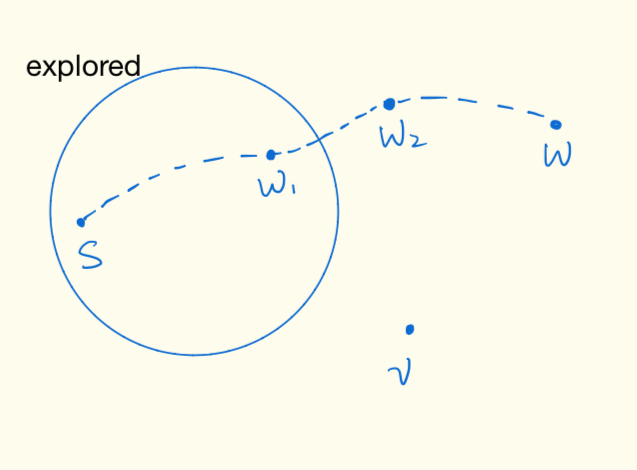
\includegraphics[scale = 0.35]{p1.png}
  \end{center}
  \tab\\
  Denote the subpath from $s$ to $w_1$ in $\Delta(s, w)$ as $p(s, w_1)$, subpath from $s$ to $w_2$ in $\Delta(s, w)$ as $p(s, w_2)$, and subpath $w_2$ to $w$ as $p(w_2, w)$. Based on \texttt{Definition 2.2 Prefix of Path}, $p(s, w_1)$ is a prefix of $\Delta(s, w)$. Since $p(s, w_1)$ is the prefix of the shortest $s-w$ path, then based on \texttt{Lemma 3.1}, $p(s, w_1)$ is the shortest path from $s$ to $w_1$, $\Delta(s, w_1) = p(s, w_1)$, $length(p(s, w_1)) = \delta(w_1)$. 
  \\
  Similarly, since $p(s, w_2) = p(s, w_1) + (w_1, w_2)$, then $p(s, w_2)$ is a prefix of $\Delta(s, w)$, and hence \texttt{Lemma 3.1} implies that $p(s, w_2)$ is the shortest path from $s$ to $w_2$. Then we have: 
  \\\\
  \ftab $\Delta(s, w_2) = p(s, w_2) = p(s, w_1) + (w_1, w_2)$ \\
  \ftab $\delta(w_2) = length(\Delta(s, w_2))$ \\
  \ftab\tab $= length(p(s, w_2))$ \\
  \ftab\tab $= length(p(s, w_1)) + weight(w_1, w_2)$\\
  \ftab\tab $= \delta(w_1) + weight(w_1, w_2)$ ([E1])
  \\
  For $\Delta(s, w)$ we have: 
  \\\\
    \tab\tsp $\delta(w) = length(p_w)$ \\
    \tab\tab $= length(p(s, w_1)) + weight(w_1, w_2) + length(p(w_2, w))$ \\
    \tab\tab $= \delta(w_1) + weight(w_1, w_2) + length(p(w_2, w))$
  \\\\
  Since all edge weights are positive, then: 
  \\\\
    \tab $\delta(w_2) = \delta(w_1) + weight(w_1, w_2) \leq \delta(w)$ ([E2])
  \\\\
  Since $w_1 \in explored_{k+2}$, there are two cases to consider: $w_1 =u_{k+1}$ and $w_1 \neq u_{k+1}$. We will prove P(k+1) under both cases below. 
  \\\\
  \texttt{Case 1: $w_1 = u_{k+1}$}
  \\
  When $w_1 = u_{k+1}$, then substitude $w_1$ by $u_{k+1}$ in [E2], we have: 
  \\\\
    \tab $\delta(w_1) + weight(w_1, w_2) = \delta(u_{k+1}) + weight(u_{k+1}, w_2) \leq delta(w)$\\
    \tab i.e.  $\delta(u_{k+1}) \leq \delta(w)$ 
  \\\\
  which contradicts with our assumption that $\delta(u_{k+1}) > \delta(w)$. Hence by the principle of prove by contradiction, $\delta(u_{k+1}) < \delta(w)$. (1) holds for P(k+1). 
  \\\\
  \texttt{Case 2}: $w_1 \neq u_{k+1}$
  \\ 
  Since $w_1 \in explored_{k+2}$ and $w_1 \neq u_{k+1}$, $w_1$ is explored before the $(k+1)^{th}$ iteration. i.e., $w_1 \in explored_{k+1}$. Suppose $w_1$ is being explored during the $i^{th}$ iteration, $i < k+1$, then based on the algorithm, the value of $dist_{i+1}[w_1]$ is calculated as: 
  \\\\
  \tab\[
        dist_{i+1}[w_1] = \left.
       \begin{cases} 
          min(dist_{i}[w_1], dist_{i}[w_1] + weight(w_1,w_1)), & (w_1,w_1) \in g \\ 
          dist_{i}[w_1] & otherwise 
        \end{cases}
        \right\}
      \]
  \\\\
  Thus $dist_{i+1}[w_1] = dist_i[w_1]$. Since the inductive hypothesis implies that $dist_{i+1}[w_1] = \delta(w_1)$, then $dist_i[w_1] = \delta(w_1)$. 
  \\
  Since $w_1$ has an edge to $w_2$, then $dist_{i+1}[w_2]$ must have been updated according as follows: 
  \\\\
  \tab\tab $dist_{i+1}[w_2] = min(dist_i[w_2], dist_i[w_1] + weight(w_1 + w_2))$ \\
  \tab\tab\tab $= min(dist_i[w_2], \delta(w_1) + weight(w_1 + w_2))$
  \\\\
  Based on [E1] we know that $\delta(w_2) =  \delta(w_1) + weight(w_1 + w_2)$, then $dist_{i+1}[w_2] = min(dist_i[w_2], \delta(w_2))$. If $dist_i[w_2] = \infty$, then $dist_{i+1}[w_2] = min(dist_i[w_2], \delta(w_2)) = \delta(w_2)$. If $dist_i[w_2] \neq \infty$, then based on \texttt{Lemma 3.2}, $dist_i[w_2]$ is the length of some $s-w_2$ path. Since $\delta(w_2) \leq length(p), \forall p \in path(s, w_2)$, then $dist_{i+1}[w_2] = min(dist_i[w_2], \delta(w_2)) = \delta(w_2)$. Hence in either cases, we conclude that $dist_{i+1}[w_2] = \delta(w_2)$. 
  \\
  Since $dist_{i+1}[w_2] = \delta(w_2)$ and $i < k+1$, then based on \texttt{Lemma 3.3}, we have $dist_{k+1}[w_2] = dist_{i+1} = \delta(w_2)$. Based on [E2], $\delta(w_2) < \delta(w)$, then $dist_{k+1}[w_2] < \delta(w)$ [NE2]. Combining with [NE1], we have: 
  \\\\
  \ftab $\delta(w) < dist_{k+1}[u_{k+1}]$ (from [NE1])\\
  \ftab $dist_{k+1}[w_2] < \delta(w)$ 
  \\\\
  Hence $dist_{k+1}[w_2] < dist_{k+1}[u_{k+1}]$ [NE2]. 
  \\
  Based on our assumption, at the beginning of the $(k+1)^{th}$ generation, $u_{k+1}, w_2 \notin explored_{k+1}$ and $u_{k+1}$ is selected by the algorithm, then we must have $dist_{k+1}[w_2] \geq dist_{k+1}[u_{k+1}]$, which contradicts with [NE2]. Hence by the principle of prove by contradiction, there does not exsist $w \in unexplored_{k+2}$, such that $\delta(u_{k+1}) > \delta(w)$, i.e. $\delta(u_{k+1}) \leq \delta(w), \forall w \in unexplored_{k+2}$. Hence (b.1) holds. 
  \\\\
  \textbf{Proof of (b.2): After the $(k+1)^{th}$ iteration, $dist_{k+1}[u_{k+1}] = \delta(u_{k+1})$}
  \\
  We will prove this by contradiction. 
  \\
  Suppose $dist_{k+1}[u_{k+1}]$ is the length of some path $p$ from $s$ to $u_{k+1}$. Assume the shortest path from $s$ to $u_{k+1}$ is some path different from $p$, i.e. $\Delta(s, u_{k+1}) \neq p$, $\delta(u_{k+1}) \leq dist_{k+1}[u_{k+1}]$([NE3]). Suppose $v'$ is the node just before $u_{k+1}$ in $\Delta(s, u_{k+1})$. 
  \\\\
  \ftab $\delta(u_{k+1}) = \delta(v') + weight(v', u_{k+1}) < dist_{k+1}[u_{k+1}]$ \\
  \tab\tab\tab Since all edge weights are non-negative, then: $\delta(v') \leq \delta(u_{k+1})$
  \\\\
  Based on (a.1) and (b.1), after the $(k+1)^{th}$ iteration, for all nodes $q \in unexplored_{k+2}$, $\delta(q) \geq \delta(u_{k+1})$, and $\delta(v') \leq \delta(u_{k+1})$, then $v'$ cannot be in $unexplored_{k+2}$. Since $unexplored_{k+1} = unexplored_{k+2} \cup u_{k+1}$, then $v' \notin unexplored_{k+1}$. Hence at the beginning of the $(k+1)^{th}$ iteration, $v'$ is already explored. Since $v'$ is explored before the $(k+1)^{th}$ iteration and $v'$ has an edge to $u_{k+1}$, then the algorithm must have considered $(\delta(v') + weight(v', u_{k+1}))$ against $dist_{k+1}[u_{k+1}]$ and chose $min((\delta(v') + weight(v', u_{k+1})), dist_{k+1}[u_{k+1}])$, which is $dist_{k+1}[u_{k+1}]$. Thus $dist_{k+1}[u_{k+1}] \leq (\delta(v') + weight(v', u_{k+1}))$, i.e. $dist_{k+1}[u_{k+1}] \leq \delta(u_{k+1})$, which contradicts with our assumption [NE3]. Hence by the principle of prove by contradiction, $dist_{k+1}[u_{k+1}] = \delta(u_{k+1})$. (b.2) holds. 
  %\end{enumerate}
\end{itemize}
Since we have proved both (1) and (2) forall nodes in $explored_{k+1}$ after the $(k+1)^{th}$ iteration, P(k+1) holds. Then by the principle of prove by induction, \texttt{Lemma 4.4} holds. 
\end{proof}